\documentclass[11pt,a4paper]{article}
\usepackage[utf8]{inputenc}
\usepackage[T1]{fontenc}
\usepackage[spanish,es-nodecimaldot]{babel}
\usepackage{lmodern}
\usepackage{geometry}
\usepackage{graphicx}
\usepackage{booktabs}
\usepackage{longtable}
\usepackage{tabularx}
\usepackage{array}
\usepackage{enumitem}
\usepackage{float}
\usepackage{xcolor}
\usepackage{hyperref}
\usepackage{fancyhdr}
\usepackage{lastpage}

\geometry{margin=2.35cm}
\hypersetup{colorlinks=true,linkcolor=blue!55!black,citecolor=blue!55!black,urlcolor=blue!55!black}
\setlength{\parskip}{0.45em}
\setlength{\parindent}{0pt}
\renewcommand{\arraystretch}{1.14}
\newcolumntype{Y}{>{\raggedright\arraybackslash}X}
\newcommand{\ruta}[1]{\texttt{\detokenize{#1}}}
\newcommand{\umdos}{\ensuremath{\mu\mathrm{m}^2}}
\newcommand{\ns}{\,ns}
\newcommand{\mhz}{\,MHz}

\pagestyle{fancy}
\fancyhf{}
\lhead{Proyecto 3 --- Arquitectura de Computadores}
\rhead{Universidad de los Andes}
\cfoot{Página \thepage\ de \pageref{LastPage}}

\begin{document}
\begin{titlepage}
\centering
\vspace*{2cm}
{\Large Universidad de los Andes\par}
\vspace{0.25cm}
{\large Facultad de Ingeniería y Ciencias Aplicadas\par}
\vspace{1.8cm}
{\Huge\bfseries Proyecto 3\par}
\vspace{0.35cm}
{\LARGE\bfseries Implementación ASIC del Pochoco SoC\par}
\vspace{0.35cm}
{\Large Juego de reflejos: RTL a GDSII con LibreLane y GF180MCU\par}
\vfill
{\large Asignatura: Arquitectura de Computadores\par}
\vspace{0.25cm}
{\large Profesor: Jorge Gómez Mir\par}
\vspace{0.9cm}
\begin{tabular}{rl}
\textbf{Integrantes:} & Christian Acevedo \\
& Guillermo Arriaza \\
& Eduardo Ponce
\end{tabular}
\vfill
{\large Semestre 2026-2\par}
{\large 24 de octubre de 2026\par}
\end{titlepage}

\begin{abstract}
Este informe documenta la adaptación del Pochoco SoC y su juego de reflejos,
originalmente implementados para una FPGA iCE40, a un macro digital ASIC con
LibreLane 3.0.16, el PDK \texttt{gf180mcuD} y la biblioteca
\texttt{gf180mcu\_fd\_sc\_mcu7t5v0}. Se implementaron dos memorias ASIC,
se realizaron síntesis, exploración de períodos, floorplanning, verificación
física y simulación post-síntesis. La referencia reglamentaria es la corrida
ROM+RAM de 100\ns{} y 40\% de utilización. Cumple setup y hold en nueve
corners y presenta DRC, LVS y antena limpios; sin embargo, conserva 2695
violaciones de slew, 10 de capacitancia y 58 de fanout. Por ello, el GDSII
generado es un candidato reproducible, no un resultado con cierre eléctrico
ni signoff definitivo.
La mejor candidata técnica posterior, \ruta{etapa12_rom_ram_no_delay_ss},
redujo las violaciones a 440 de slew, 2 de capacitancia y 57 de fanout.
La Etapa 21 finalmente alcanzó cero violaciones eléctricas en el macro
con la corrida \ruta{etapa21_combined}; el GDSII sigue siendo candidato de
macro y no certifica un chip completo con pads e I/O.
\end{abstract}

\tableofcontents
\newpage

\section{Introducción y objetivo}
El objetivo fue llevar el repositorio del grupo entregado en el Proyecto 2 ---RTL modificado, \ruta{game.s} y assembler--- desde FPGA hasta una implementación ASIC. El resultado es un macro digital con terminales lógicos, no un chip completo con pad ring, ESD, encapsulado ni caracterización de I/O.

Las decisiones se sustentan en corridas preservadas dentro de \ruta{asic/runs/}, sus \ruta{flow.log}, \ruta{resolved.json}, reportes de STA y \ruta{final/metrics.json}. La documentación oficial describe metodología, PDK y herramientas; no se usa para sustituir datos experimentales.

\section{Arquitectura del Pochoco SoC y adaptación FPGA--ASIC}
\subsection{Arquitectura original}
El sistema integra el procesador Espino RV32E, register file, ALU, controlador, memoria, periféricos del juego, SPI, cuatro botones, cuatro LED y dos displays de siete segmentos. El juego conserva diez rondas, contabiliza la respuesta y calcula el promedio.

\begin{figure}[H]
\centering
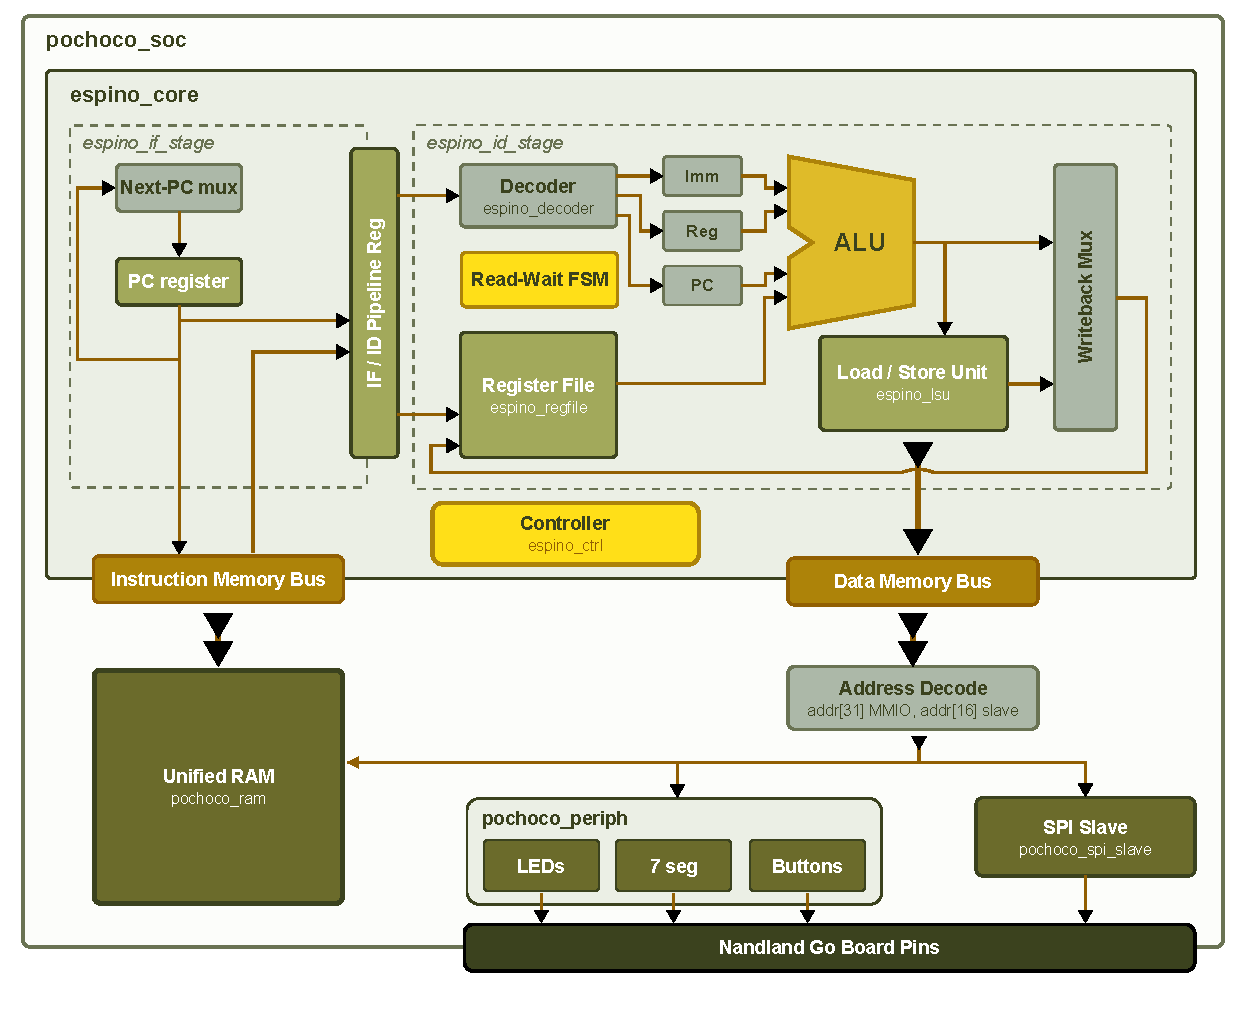
\includegraphics[width=0.86\linewidth]{figuras/pochoco_soc.pdf}
\caption{Arquitectura lógica existente del Pochoco SoC: Espino, memoria, periféricos del juego y SPI. Es un diagrama RTL, no una vista física.}
\label{fig:pochoco}
\end{figure}

\subsection{Separación del top ASIC}
Se creó \ruta{rtl/asic_top.v}, que instancia el SoC y expone \ruta{clk_i}, \ruta{rst_ni}, \ruta{btn_i[3:0]}, \ruta{leds_o[3:0]}, los dos buses de siete segmentos y SPI. No contiene restricciones de pines. El top FPGA \ruta{rtl/game_top.v} se preservó y sigue generando su reset de power-on de 2048 ciclos.

Para ASIC, \ruta{rtl/pochoco_soc.v} recibe reset externo activo bajo \ruta{i_Rst_ni}; se eliminó del camino ASIC el contador de power-on propio de iCE40. La Tabla \ref{tab:fpga-asic} resume las incompatibilidades tratadas.

\begin{table}[H]
\centering\small
\caption{Dependencias FPGA y reemplazo ASIC.}
\label{tab:fpga-asic}
\begin{tabularx}{\linewidth}{p{0.25\linewidth}YY}
\toprule
Construcción FPGA & Problema ASIC & Tratamiento aplicado \\
\midrule
\ruta{SB_RAM40_4K} e inferencia BRAM & Primitiva iCE40 sin equivalente GF180 & Excluida de fuentes ASIC; reemplazada por memorias FF/ROM. \\
\ruta{\$readmemh} e \ruta{initial} & No existe un archivo cargado al encender silicio & Programa incorporado en \ruta{game_rom.v} generado por assembler. \\
Power-on reset interno & Depende de arranque FPGA & \ruta{asic_top.v} recibe reset externo; \ruta{game_top.v} conserva FPGA. \\
\ruta{.pcf} & Son pines de placa, no terminales de macro & No se usan en la configuración ASIC. \\
\bottomrule
\end{tabularx}
\end{table}

El debounce fue parametrizado para preservar FPGA y definir el valor ASIC. El valor histórico de 249999 ciclos es 10\,ms a 25\mhz{}, pero 25\,ms a 10\mhz{}; esta diferencia quedó documentada sin alterar las diez rondas.

\subsection{Evidencia del flujo para la adaptación}
Los constructos FPGA no se sometieron intencionalmente a la síntesis ASIC. El
\ruta{resolved.json} de \ruta{etapa9_rom_ram_util40_debounce} enumera
\ruta{espino_register_file_ff.v}, \ruta{pochoco_memory_rom_ram.v} y
\ruta{game_rom.v}, pero no \ruta{espino_register_file.v} ni
\ruta{pochoco_ram.v}. Por ello no existe un warning de LibreLane sobre
\ruta{SB_RAM40_4K}, \ruta{\$readmemh} o \ruta{initial}: la ausencia del
mensaje se debe a su exclusión deliberada, no a que sean construcciones ASIC
aceptadas.

La evidencia real del flujo es la siguiente. En
\ruta{06-yosys-synthesis/yosys-synthesis.log:145--146}, Yosys advierte
``Replacing memory \texttt{bank\_b} / \texttt{bank\_a} with list of
registers'' y apunta a
\ruta{rtl/espino_core/espino_register_file_ff.v:23} y :22, respectivamente;
esto confirma que la alternativa ASIC se implementa con registros
sintetizables. En
\ruta{warning.log:2--3}, LibreLane informa que \ruta{PNR_SDC_FILE} y
\ruta{SIGNOFF_SDC_FILE} no están definidos y usa la SDC genérica. Este warning
es real y limita la interpretación de timing de interfaz; no es una advertencia
de compatibilidad FPGA. Los warnings de biblioteca \ruta{STA-1140} y de LEF58
en \ruta{warning.log:4--30} son de herramienta/PDK y tampoco evidencian una
dependencia FPGA.

\section{Arquitecturas de memoria y extensión del assembler}
\subsection{Uso real del programa}
El assembler analiza \ruta{sw/game.s} y produce una imagen de 143 instrucciones (572 bytes). El juego usa una palabra de datos no-MMIO en \ruta{0x7FC}; los periféricos se direccionan separadamente. Espino espera lectura registrada.

\begin{table}[H]
\centering\small
\caption{Arquitecturas de memoria ASIC implementadas.}
\label{tab:memory}
\setlength{\tabcolsep}{4pt}
\begin{tabularx}{\linewidth}{>{\raggedright\arraybackslash}p{0.18\linewidth}>{\raggedright\arraybackslash}p{0.38\linewidth}>{\raggedright\arraybackslash}p{0.38\linewidth}}
\toprule
Característica & ROM combinacional + RAM reducida & Memoria unificada con flip-flops \\
\midrule
Selección & \shortstack[l]{\texttt{MemoryArchitecture}\\\texttt{=1}} & \shortstack[l]{\texttt{MemoryArchitecture}\\\texttt{=2}} \\
Programa & \ruta{game_rom}: 143 palabras mediante \ruta{case} & 144 palabras: 143 de programa y una de datos \\
Datos & Registro de 32 bits en \ruta{0x7FC}; escritura por byte & Última palabra del arreglo unificado \\
Inicialización & Lógica incorporada; sin \ruta{initial} & Copia hardware desde ROM y reset retenido \\
Archivo al encender & No depende de \ruta{game.hex} & No depende de \ruta{game.hex} \\
\bottomrule
\end{tabularx}
\setlength{\tabcolsep}{6pt}
\end{table}

El assembler se extendió para generar tanto \ruta{game.hex} como \ruta{asic/generated/game_rom.v}. Los targets del Makefile regeneran ambos artefactos desde \ruta{game.s}; el programa fuente no fue modificado.

\begin{table}[H]
\centering\small
\caption{Comparación de memorias. Área y FF: síntesis; die y utilización: post-route.}
\label{tab:memory-results}
\begin{tabular}{lrr}
\toprule
Métrica & ROM+RAM & Unificada FF \\
\midrule
Palabras de programa / datos & 143 / 1 & 143 / 1 (144 físicas) \\
Área Yosys (\umdos{}) & 142038,2208 & 566548,1920 \\
Flip-flops mapeados & 874 & 5317 \\
Celdas sintetizadas & 5140 & 17660 \\
Área stdcell post-route (\umdos{}) & 184179 & 730205 \\
Área de die (mm$^2$) & 0,382215 & 1,470110 \\
Utilización física & 51,8778\% & 51,6617\% \\
Menor período demostrado & 62\ns{} & 100\ns{} \\
Frecuencia demostrada & 16,129\mhz{} & 10\mhz{} (no máximo probado) \\
\bottomrule
\end{tabular}
\end{table}

ROM+RAM se eligió como candidata por usar aproximadamente cuatro veces menos área de síntesis. La frecuencia de la unificada se informa como demostrada, no como máximo, porque no se hizo un barrido adicional.

\section{Síntesis, celdas más utilizadas y desglose jerárquico}
Las corridas usaron LibreLane 3.0.16, PDK \ruta{gf180mcuD} revisión \ruta{8afc8346a57fe1ab7934ba5a6056ea8b43078e71}, biblioteca \ruta{gf180mcu_fd_sc_mcu7t5v0} y Yosys 0.62. La comparación inicial produjo 140802,3232\umdos{} y 874 FF para ROM+RAM, frente a 565735,9680\umdos{} y 5317 FF para memoria unificada.

\begin{table}[H]
\centering\small
\caption{Cinco celdas estándar más usadas en la corrida reglamentaria.}
\label{tab:cells}
\begin{tabularx}{\linewidth}{p{0.35\linewidth}rY}
\toprule
Celda & Cantidad & Función y explicación \\
\midrule
\ruta{dffrnq_1} & 871 & Estado secuencial; 544 FF del register file, 142 de periféricos y 96 de memoria ROM+RAM. \\
\ruta{nand2_1} & 841 & Red booleana aplanada: decodificación ROM, muxes y control. \\
\ruta{oai21_1} & 588 & Selectores y condiciones compuestas. \\
\ruta{nor2_1} & 452 & Decodificación, comparación y control. \\
\ruta{aoi21_1} & 409 & Selectores, comparaciones y reducción lógica. \\
\bottomrule
\end{tabularx}
\end{table}

La síntesis de diagnóstico preservó jerarquía antes del aplanamiento. Así no se atribuye área por suposición cuando ABC elimina nombres internos.

\begin{table}[H]
\centering\small
\caption{Áreas jerárquicas diagnosticadas.}
\label{tab:hier-area}
\begin{tabular}{lrrl}
\toprule
Elemento & Área (\umdos{}) & Fracción & Método \\
\midrule
Register file \ruta{espino_register_file_ff} & 69071,9680 & 48,668\% & Módulo hoja preservado \\
ALU \ruta{espino_alu} & 7448,3136 & 5,248\% & Módulo hoja preservado \\
Contador \ruta{cycle_q} & 3714,2784 & 2,617\% & Cono inverso de 97 celdas \\
ROM \ruta{game_rom} & 9568,8768 & 6,742\% & Módulo hoja preservado \\
Periférico completo & 17436,4736 & 12,286\% & Estadística jerárquica \\
SoC total & 141924,0704 & 100\% & \ruta{stat} con Liberty \\
\bottomrule
\end{tabular}
\end{table}

Se esperaba cualitativamente que la unificada fuera mayor por almacenar el programa en FF, lo que se confirmó. No existía predicción numérica previa; no se construye una estimación retrospectiva. El register file dominó el área.

\section{Análisis de timing y ruta crítica}
\subsection{Barrido de período}
La arquitectura ROM+RAM se evaluó a 100, 70, 62 y 60\ns{}. En las corridas sin slack negativo LibreLane reporta WNS=0 y TNS=0; por claridad se muestra además el peor slack real (WS). Cada período induce una nueva optimización, placement y buffering.

La Tabla \ref{tab:timing-100} transcribe las métricas de
\ruta{etapa4_rom_ram_100ns_100/55-openroad-stapostpnr/state_out.json}. El
corner típico es \ruta{nom_tt_025C_5v00} y el más lento para setup es
\ruta{max_ss_125C_4v50}. Aquí \emph{WNS}=0 no significa slack nulo: LibreLane
trunca el total de slack negativo a cero cuando no existen violaciones. Por
ello, WS conserva el margen positivo real que se usa para comparar rutas.

\begin{table}[H]
\centering\footnotesize
\caption{STA post-route ROM+RAM a 100\ns{}: WNS, TNS y peor slack real (WS).}
\label{tab:timing-100}
\begin{tabular}{lrrr rrr}
\toprule
Corner & \multicolumn{3}{c}{Setup (ns)} & \multicolumn{3}{c}{Hold (ns)} \\
\cmidrule(lr){2-4}\cmidrule(lr){5-7}
& WNS & TNS & WS & WNS & TNS & WS \\
\midrule
Típico: \ruta{nom_tt_025C_5v00} & 0 & 0 & +67,579189 & 0 & 0 & +0,384634 \\
Lento: \ruta{max_ss_125C_4v50} & 0 & 0 & +38,023054 & 0 & 0 & +0,964812 \\
\bottomrule
\end{tabular}
\end{table}

\begin{table}[H]
\centering\small
\caption{Barrido ROM+RAM: corners representativos y resultado de nueve corners.}
\label{tab:sweep}
\begin{tabular}{rrrrrl}
\toprule
Período & WS típico & WS setup lento & TNS setup lento & WS hold lento & Resultado \\
(ns) & (ns) & (ns) & (ns) & (ns) & \\
\midrule
100 & +67,579 & +38,023 & 0 & +0,965 & Cumple \\
70 & +37,579 & +8,023 & 0 & +0,965 & Cumple \\
62 & +29,579 & +0,023 & 0 & +0,965 & Cumple; mínimo demostrado \\
60 & +27,579 & -1,977 & -26,791 & +0,965 & Falla setup \\
\bottomrule
\end{tabular}
\end{table}

El menor período que cerró los nueve corners fue 62\ns{}, equivalente a 16,129\mhz{}. La ruta crítica de 100\ns{} en \ruta{max_ss_125C_4v50} parte de \ruta{_8522_} (\ruta{a_rdata_o[3]}) y termina en \ruta{_8510_} (\ruta{a_addr_i[25]} del PC). Corresponde a \emph{fetch} $\rightarrow$ decode/ejecución de salto $\rightarrow$ actualización de PC. El reporte \ruta{max.rpt} de Etapa 4 conserva celdas, buffers y retardos.

\section{Optimización RTL y resultados comparativos}
\subsection{ALU experimental}
Se propuso calcular comparaciones de igualdad y menor-que en paralelo con el sumador/restador. No modificó ciclos visibles, pero a 60\ns{} aumentó lógica y desplazó la ruta crítica hacia fetch/decode. Por ello fue descartada y nunca se usó en la referencia física.

\begin{table}[H]
\centering\small
\caption{Resultado de la optimización experimental de ALU a 60\ns{}.}
\label{tab:aluopt}
\begin{tabular}{lrrr}
\toprule
Variante & WNS/TNS setup lento (ns) & Placement (\umdos{}) & Stdcell post-route (\umdos{}) \\
\midrule
Baseline & -1,977 / -26,791 & 153524 & 184179 \\
ALU experimental & -7,069 / -264,994 & 155010 & 186348 \\
\bottomrule
\end{tabular}
\end{table}

\subsection{Experimento localizado de Etapa 10}
El análisis eléctrico mostró campos registrados de instrucción alimentando selectores del register file; las violaciones de fanout se concentraron en CTS. Se probó un register file en cuatro bancos de 8 bits sin agregar etapas ni cambiar el ISA. La comparación ciclo a ciclo produjo \ruta{mismatches=0}, pero slew pasó de 2695 a 3055 y capacitancia de 10 a 23. Su peor slack setup bajó de +37,171987 a +31,409535\ns{}; la variante se descarta.

\section{Cálculo de las constantes temporales del juego a 100\ns{}}
El reloj ASIC reglamentario es 10\mhz{} porque $T=100\ns$. Por tanto:
\[
N_{3\,s}=\frac{3\,s}{100\,ns}=30\,000\,000,\qquad
N_{0,1\,s}=\frac{0,1\,s}{100\,ns}=1\,000\,000.
\]
Las constantes ASIC se incorporaron en \ruta{sw/game_asic_100ns.s} y se regeneró la ROM de 143 palabras. La versión para FPGA de \ruta{game.s} se preservó; la configuración de compilación separa ambas imágenes.

\section{Floorplan, alimentación, placement y terminales}
La documentación de LibreLane organiza configuraciones JSON reproducibles y preserva estados por paso~\cite{librelane_docs}. OpenROAD inicializa floorplan a partir de área y utilización, realiza placement, CTS, routing y extracción RC~\cite{openroad_docs}. El PDK provee las vistas tecnológicas y la biblioteca estándar de siete tracks~\cite{gf180mcu_pdk_docs}.

% Integra explícitamente el fragmento de citas preparado en la revisión oficial.
% Fragmento integrado desde main.tex con % Fragmento integrado desde main.tex con % Fragmento integrado desde main.tex con \input{citas_oficiales.tex}.
% Para BibTeX clásico, agregar al final del informe:
% \bibliographystyle{IEEEtran}
% \bibliography{referencias}
%
% Con biblatex, usar en el preámbulo:
% \addbibresource{referencias.bib}
% y \printbibliography en lugar de los dos comandos anteriores.

\subsection{Flujo RTL a GDSII con LibreLane}
La implementación ASIC se ejecutó con LibreLane 3.0.16 en Docker/WSL. LibreLane
acepta configuraciones JSON validadas y organiza un flujo reproducible de
implementación digital desde RTL hasta las vistas físicas. La configuración
reglamentaria usa \texttt{DESIGN\_NAME=asic\_top}, \texttt{CLOCK\_PORT=clk\_i},
\texttt{CLOCK\_PERIOD=100 ns} y \texttt{FP\_CORE\_UTIL=40}.
La documentación oficial se usa para describir el flujo y sus parámetros;
las métricas de este proyecto provienen exclusivamente de sus logs y reportes
originales~\cite{librelane_docs}.

\subsection{Tecnología GF180MCU y biblioteca estándar}
El flujo utiliza la variante instalada \texttt{gf180mcuD}, correspondiente a
la familia de tecnología GF180MCU, con la revisión de \texttt{open\_pdks}
\texttt{8afc8346a57fe1ab7934ba5a6056ea8b43078e71}. La biblioteca seleccionada
es \texttt{gf180mcu\_fd\_sc\_mcu7t5v0}, una biblioteca estándar de siete
tracks documentada por el PDK. Esta referencia respalda la procedencia de las
vistas tecnológicas y de celdas, no reemplaza la revisión exacta registrada en
las corridas~\cite{gf180mcu_pdk_docs}.

\subsection{Implementación física y análisis de timing con OpenROAD}
LibreLane invoca OpenROAD para inicialización del floorplan, placement, CTS,
routing, extracción RC y STA post-route. El uso de utilización para dimensionar
el core, la inspección de congestión y el análisis después de extracción son
coherentes con las capacidades documentadas de OpenROAD~\cite{openroad_docs}.
Los valores de WNS, TNS, DRC, LVS, antena y violaciones eléctricas presentados
en este informe se toman de los reportes originales de LibreLane/OpenROAD; no
se deducen de esta documentación.
.
% Para BibTeX clásico, agregar al final del informe:
% \bibliographystyle{IEEEtran}
% \bibliography{referencias}
%
% Con biblatex, usar en el preámbulo:
% \addbibresource{referencias.bib}
% y \printbibliography en lugar de los dos comandos anteriores.

\subsection{Flujo RTL a GDSII con LibreLane}
La implementación ASIC se ejecutó con LibreLane 3.0.16 en Docker/WSL. LibreLane
acepta configuraciones JSON validadas y organiza un flujo reproducible de
implementación digital desde RTL hasta las vistas físicas. La configuración
reglamentaria usa \texttt{DESIGN\_NAME=asic\_top}, \texttt{CLOCK\_PORT=clk\_i},
\texttt{CLOCK\_PERIOD=100 ns} y \texttt{FP\_CORE\_UTIL=40}.
La documentación oficial se usa para describir el flujo y sus parámetros;
las métricas de este proyecto provienen exclusivamente de sus logs y reportes
originales~\cite{librelane_docs}.

\subsection{Tecnología GF180MCU y biblioteca estándar}
El flujo utiliza la variante instalada \texttt{gf180mcuD}, correspondiente a
la familia de tecnología GF180MCU, con la revisión de \texttt{open\_pdks}
\texttt{8afc8346a57fe1ab7934ba5a6056ea8b43078e71}. La biblioteca seleccionada
es \texttt{gf180mcu\_fd\_sc\_mcu7t5v0}, una biblioteca estándar de siete
tracks documentada por el PDK. Esta referencia respalda la procedencia de las
vistas tecnológicas y de celdas, no reemplaza la revisión exacta registrada en
las corridas~\cite{gf180mcu_pdk_docs}.

\subsection{Implementación física y análisis de timing con OpenROAD}
LibreLane invoca OpenROAD para inicialización del floorplan, placement, CTS,
routing, extracción RC y STA post-route. El uso de utilización para dimensionar
el core, la inspección de congestión y el análisis después de extracción son
coherentes con las capacidades documentadas de OpenROAD~\cite{openroad_docs}.
Los valores de WNS, TNS, DRC, LVS, antena y violaciones eléctricas presentados
en este informe se toman de los reportes originales de LibreLane/OpenROAD; no
se deducen de esta documentación.
.
% Para BibTeX clásico, agregar al final del informe:
% \bibliographystyle{IEEEtran}
% \bibliography{referencias}
%
% Con biblatex, usar en el preámbulo:
% \addbibresource{referencias.bib}
% y \printbibliography en lugar de los dos comandos anteriores.

\subsection{Flujo RTL a GDSII con LibreLane}
La implementación ASIC se ejecutó con LibreLane 3.0.16 en Docker/WSL. LibreLane
acepta configuraciones JSON validadas y organiza un flujo reproducible de
implementación digital desde RTL hasta las vistas físicas. La configuración
reglamentaria usa \texttt{DESIGN\_NAME=asic\_top}, \texttt{CLOCK\_PORT=clk\_i},
\texttt{CLOCK\_PERIOD=100 ns} y \texttt{FP\_CORE\_UTIL=40}.
La documentación oficial se usa para describir el flujo y sus parámetros;
las métricas de este proyecto provienen exclusivamente de sus logs y reportes
originales~\cite{librelane_docs}.

\subsection{Tecnología GF180MCU y biblioteca estándar}
El flujo utiliza la variante instalada \texttt{gf180mcuD}, correspondiente a
la familia de tecnología GF180MCU, con la revisión de \texttt{open\_pdks}
\texttt{8afc8346a57fe1ab7934ba5a6056ea8b43078e71}. La biblioteca seleccionada
es \texttt{gf180mcu\_fd\_sc\_mcu7t5v0}, una biblioteca estándar de siete
tracks documentada por el PDK. Esta referencia respalda la procedencia de las
vistas tecnológicas y de celdas, no reemplaza la revisión exacta registrada en
las corridas~\cite{gf180mcu_pdk_docs}.

\subsection{Implementación física y análisis de timing con OpenROAD}
LibreLane invoca OpenROAD para inicialización del floorplan, placement, CTS,
routing, extracción RC y STA post-route. El uso de utilización para dimensionar
el core, la inspección de congestión y el análisis después de extracción son
coherentes con las capacidades documentadas de OpenROAD~\cite{openroad_docs}.
Los valores de WNS, TNS, DRC, LVS, antena y violaciones eléctricas presentados
en este informe se toman de los reportes originales de LibreLane/OpenROAD; no
se deducen de esta documentación.


\begin{figure}[H]
\centering
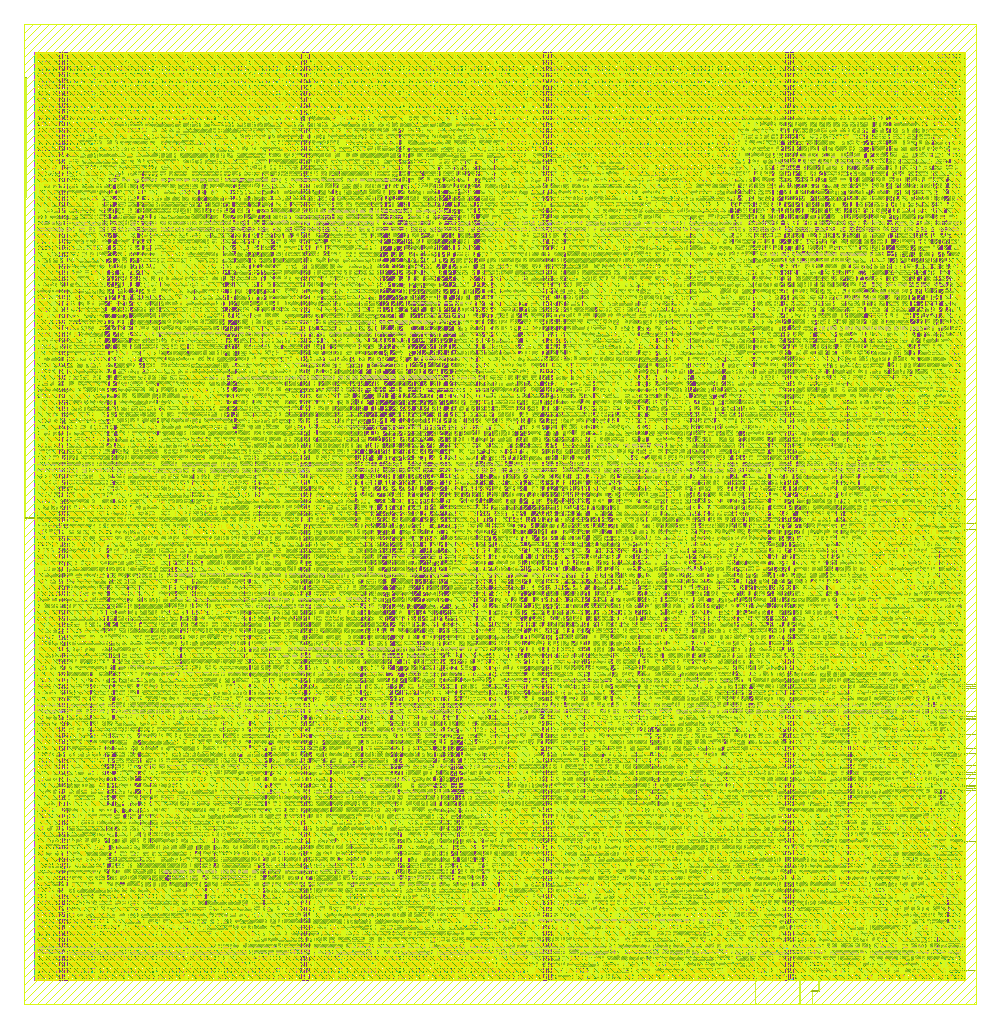
\includegraphics[width=0.76\linewidth]{figuras/etapa9_render.png}
\caption{Vista física real del macro \ruta{asic_top} en la corrida reglamentaria de Etapa 9 (100\ns{}, 40\%). El contorno corresponde al die y el interior a las celdas/rutas implementadas; la imagen no representa pads de encapsulado ni demuestra cierre eléctrico.}
\label{fig:stage9-render}
\end{figure}

La red PDN usa \ruta{VDD} y \ruta{VSS}: rails Metal1, straps verticales Metal4 y horizontales Metal5. Las conexiones globales enlazan \ruta{VDD}/\ruta{VNW} y \ruta{VSS}/\ruta{VPW} de las celdas. El flujo reportó cero violaciones de conectividad de malla; el IR drop no es signoff de chip porque no se definieron \ruta{VSRC_LOC_FILES}.

Los terminales fueron colocados automáticamente, sin \ruta{FP_PIN_ORDER_CFG}. \ruta{clk_i} quedó en el borde izquierdo superior, \ruta{rst_ni} en el derecho inferior y SPI, botones, LED y displays principalmente en el borde derecho. Son terminales de macro, no un pinout de encapsulado: un chip completo requeriría pads, ESD y drivers de carga.

\begin{figure}[H]
\centering
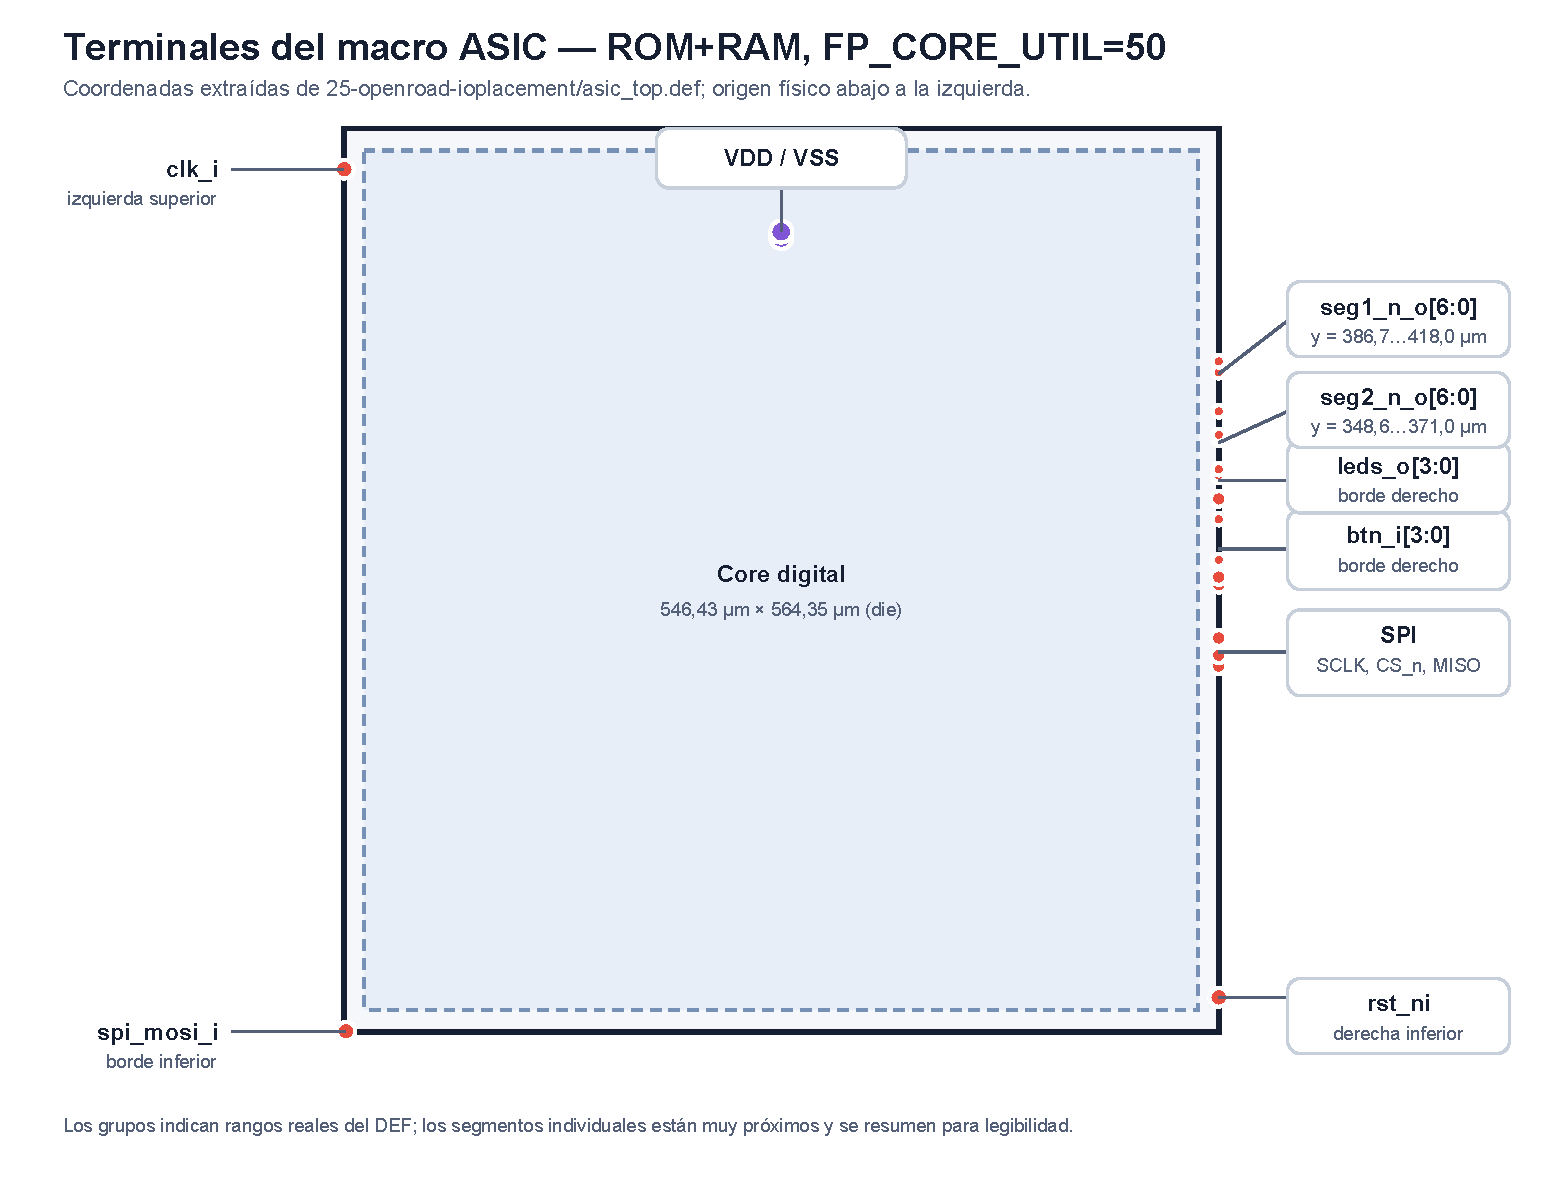
\includegraphics[width=0.92\linewidth]{figuras/etapa5_pinout_util50.pdf}
\caption{Mapa de terminales lógicos sobre el borde del macro en la corrida de 50\% de Etapa 5. Identifica reloj, reset, SPI, botones, LED, displays, VDD y VSS. La ubicación fue automática, por lo que esta figura describe el placement observado y no un pinout de paquete impuesto.}
\label{fig:pinout}
\end{figure}

\section{Exploración de utilización y cálculo de costos}
\subsection{Tres floorplans}
\begin{table}[H]
\centering\small
\caption{Exploración física de utilización. Área de celdas y área de die se distinguen.}
\label{tab:util}
\setlength{\tabcolsep}{3pt}
\begin{tabularx}{\linewidth}{>{\centering\arraybackslash}p{0.07\linewidth}>{\raggedleft\arraybackslash}p{0.12\linewidth}>{\centering\arraybackslash}p{0.17\linewidth}>{\centering\arraybackslash}p{0.08\linewidth}>{\centering\arraybackslash}p{0.16\linewidth}>{\centering\arraybackslash}p{0.21\linewidth}>{\centering\arraybackslash}p{0.07\linewidth}}
\toprule
\shortstack{Objetivo\\(\%)} & \shortstack{Área stdcell\\(\umdos{})} & \shortstack{Core / die\\(mm$^2$)} & \shortstack{Uso GRT\\(\%)} & \shortstack{Slew / cap.\\/ fanout} & \shortstack{DRC / Magic\\/ LVS / antena} & Cierre \\
\midrule
30 & 187986 & 0,471748 / 0,504709 & 20,49 & 3364 / 26 / 58 & 0 / 0 / 0 / 0 & No \\
40 & 184179 & 0,355025 / 0,382215 & 24,78 & 3008 / 31 / 56 & 0 / 0 / 0 / 0 & No \\
50 & 181532 & 0,281831 / 0,308378 & 28,64 & 2400 / 1 / 55 & 0 / 0 / 0 / 0 & No \\
\bottomrule
\end{tabularx}
\setlength{\tabcolsep}{6pt}
\end{table}

\begin{figure}[H]
\centering
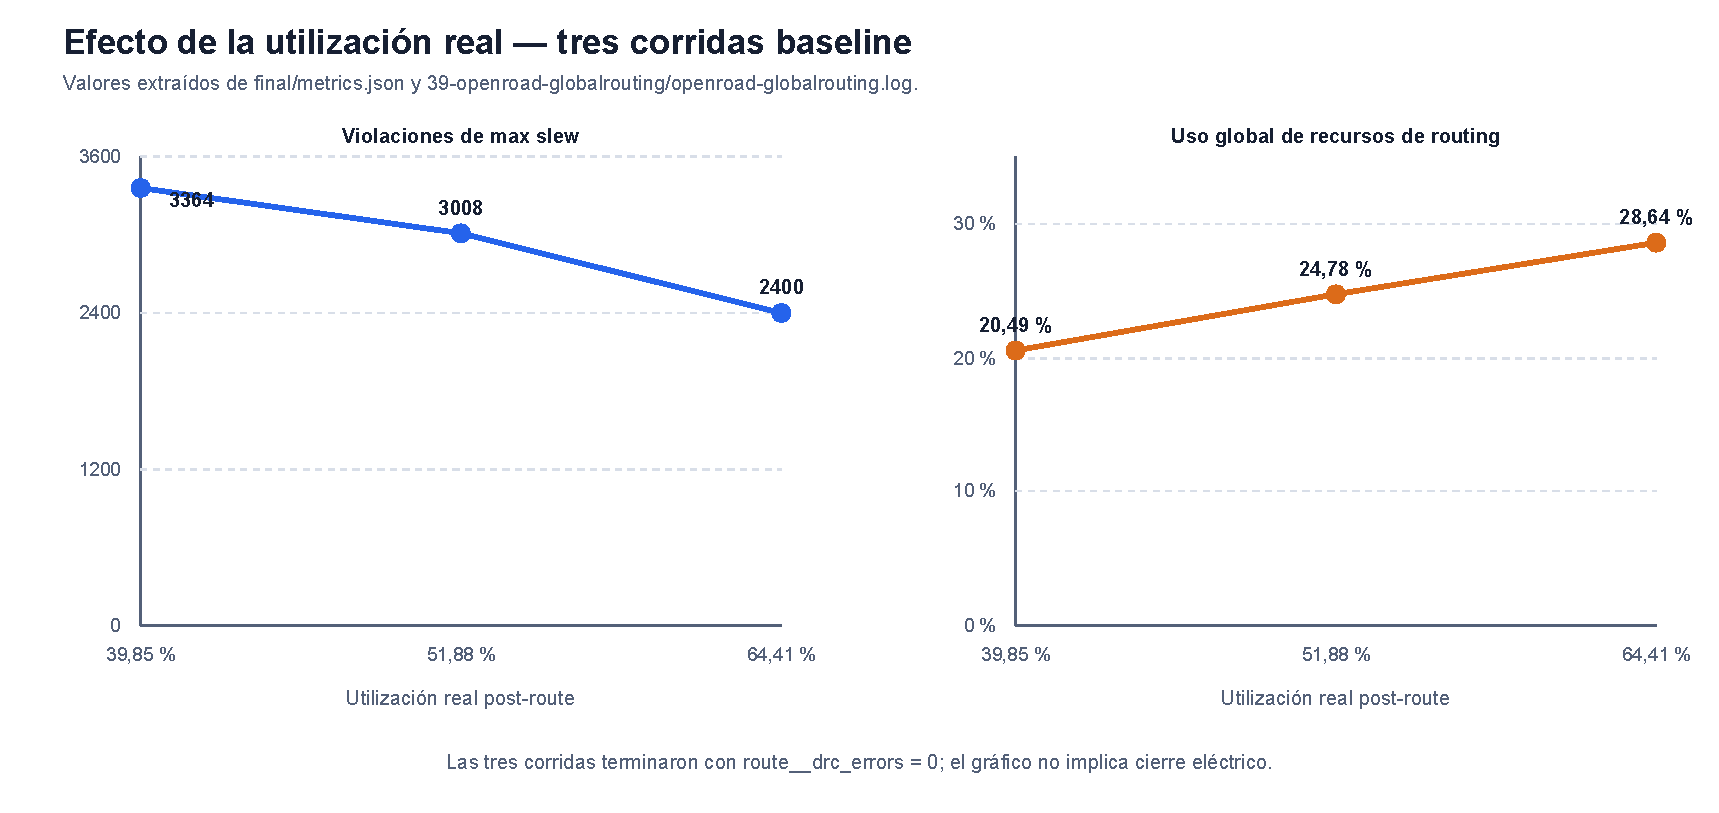
\includegraphics[width=0.90\linewidth]{figuras/etapa5_utilizacion.pdf}
\caption{Datos reales de Etapa 5 para 30\%, 40\% y 50\% de \ruta{FP_CORE_UTIL}; relaciona utilización objetivo con la métrica de violaciones/congestión reportada. Ningún punto del gráfico constituye cierre eléctrico.}
\label{fig:utilplot}
\end{figure}

El menor die probado fue 0,308378\,mm$^2$ a 50\%, pero no es mínimo válido de cierre porque ninguna corrida eliminó sus violaciones eléctricas. La baseline reglamentaria posterior de Etapa 9 se mantiene a 40\% y tiene die de 0,375554\,mm$^2$, debido a la configuración actualizada con debounce.

\subsection{Costo académico}
Aplicando la referencia de US\$23000/mm$^2$ al die reglamentario:
\[
0,375554\ \mathrm{mm}^2 \times \mathrm{US\$}23000/\mathrm{mm}^2 = \mathrm{US\$}8637,74.
\]
Es un ejercicio académico lineal. Omite NRE, máscaras, yield, área de pads, encapsulado, test, volumen, obleas y costos de fabricación. ROM+RAM reduce el costo relativo al evitar miles de FF de la memoria unificada.

\section{DRC, LVS, antena y análisis eléctrico}
\subsection{Configuración reglamentaria y STA}
La referencia principal es \ruta{etapa9_rom_ram_util40_debounce}: ROM+RAM, 100\ns{}, \ruta{FP_CORE_UTIL=40}, die de 0,375554\,mm$^2$. En nueve corners, el peor slack setup es +37,171987\ns{} en \ruta{max_ss_125C_4v50} y el peor hold es +0,126038\ns{} en \ruta{min_ff_n40C_5v50}; TNS de setup y hold es cero.

\begin{table}[H]
\centering\small
\caption{Estado físico de la corrida reglamentaria de Etapa 9.}
\label{tab:stage9}
\begin{tabularx}{\linewidth}{lY}
\toprule
Propiedad & Resultado real \\
\midrule
Área core / die & 0,347061 / 0,375554 mm$^2$ \\
Utilización stdcell & 52,2176\% \\
Setup / hold, nueve corners & Peor slack +37,171987 / +0,126038\ns{}; TNS=0 / 0 \\
Routing DRC / Magic DRC / LVS / antena / XOR & 0 / 0 / 0 / 0 / 0 \\
KLayout DRC externo & Limpio con deck GF180MCU instalado \\
Slew / capacitancia / fanout & 2695 / 10 / 58 en el peor conteo \\
Estado & Flujo completo, sin cierre eléctrico \\
\bottomrule
\end{tabularx}
\end{table}

La SDC empleada es la genérica de LibreLane: no se definieron \ruta{PNR_SDC_FILE} ni \ruta{SIGNOFF_SDC_FILE} para una interfaz ASIC completa. El timing es válido bajo esas restricciones, pero no representa delays, transiciones o cargas de pads/package reales.

\subsection{Reparaciones dirigidas de las Etapas 12 a 21}
La corrida reglamentaria de Etapa 9 se conserva como referencia obligatoria
de 100\ns{} y 40\%. Los experimentos posteriores mantuvieron ese período,
la utilización objetivo, la arquitectura ROM+RAM y la misma biblioteca.
La Etapa 12 excluyó la familia de celdas de delay en el sizing y ejecutó
la reparación en el corner SS; el sintetizado funcional se mantuvo
idéntico. La Etapa 13 probó por separado un ajuste post-GRT de datos y
una redistribución de cargas del árbol de reloj (CTS). Los recuentos
comparables del peor corner eléctrico se muestran en el
Cuadro~\ref{tab:repair-electrical}. La evidencia original está en
\ruta{reports/stage12/comparison.csv} y
\ruta{reports/stage13/comparison.csv}; las tablas de nueve corners están
en \ruta{reports/stage12/timing_nine_corners.csv} y
\ruta{reports/stage13/timing_nine_corners.csv}.

\begin{table}[H]
\centering\small
\caption{Comparación eléctrica post-route; los valores son recuentos de violaciones, no magnitudes de transición.}
\label{tab:repair-electrical}
\begin{tabularx}{\linewidth}{Yrrr}
\toprule
Corrida / condición & Slew & Capacitancia & Fanout \\
\midrule
Etapa 9, reglamentaria & 2695 & 10 & 58 \\
Etapa 12, reparación SS & 440 & 2 & 57 \\
Etapa 13, datos post-GRT & 410 & 3 & 57 \\
Etapa 13, CTS redistribuido & 468 & 1 & 0 \\
\bottomrule
\end{tabularx}
\end{table}

\begin{table}[H]
\centering\footnotesize
\caption{Área física y peor slack real post-route. \emph{WS} es la holgura positiva medida; LibreLane informa WNS/TNS = 0/0\ns{} al truncar WNS no negativo.}
\label{tab:repair-physical}
\begin{tabularx}{\linewidth}{Yrrrr}
\toprule
Corrida & Celdas (\umdos) & Die (mm$^2$) & Setup WS (ns) & Hold WS (ns) \\
\midrule
Etapa 9 & 181227 & 0,375554 & +37,171987 & +0,126038 \\
Etapa 12 SS & 177912 & 0,375554 & +53,646852 & +0,054793 \\
Etapa 13 post-GRT & 177917 & 0,375554 & +53,159008 & +0,054793 \\
Etapa 13 CTS & 186061 & 0,375554 & +52,430605 & +0,010418 \\
\bottomrule
\end{tabularx}
\end{table}

\begin{table}[H]
\centering\footnotesize
\caption{Métricas finales de la corrida de cierre eléctrico Etapa 21.}
\label{tab:stage21-final}
\begin{tabularx}{\linewidth}{YrrrY}
\toprule
Métrica & Valor & Unidad & Evidencia & Estado \\
\midrule
CLOCK\_PERIOD & 100 & ns & \ruta{asic/rom_ram_stage21_combined.json} & configurado \\
FP\_CORE\_UTIL & 40 & \% & \ruta{asic/rom_ram_stage21_combined.json} & configurado \\
Área de celdas & 187808 & \umdos & \ruta{asic/runs/etapa21_combined/final/metrics.json} & reportada \\
Utilización & 0,541139 & -- & \ruta{asic/runs/etapa21_combined/final/metrics.json} & reportada \\
Slew / capacitancia / fanout & 0 / 0 / 0 & violaciones & STA post-route con SPEF & cumplido \\
Setup / hold WNS peor & +53,053929 / +0,006720 & ns & nueve corners & cumplido \\
DRC / Magic / LVS / antena / XOR & 0 / 0 / 0 / 0 / limpio & errores & reportes de la corrida & limpio \\
KLayout DRC externo / PDN & limpio / conectado & -- & \ruta{reports/stage21_etapa21_combined.lyrdb} e IR drop & verificado \\
\bottomrule
\end{tabularx}
\end{table}

En las cuatro corridas completas, setup y hold tienen WNS/TNS de
0/0\ns{} en los nueve corners. El routing DRC, Magic DRC, LVS y antena
terminaron sin errores en los experimentos completos; KLayout DRC externo
fue ejecutado y quedó limpio para Etapa 9, para la candidata de Etapa 12 y
para \ruta{etapa21_combined},
\emph{no} para las dos variantes de Etapa 13. Los reportes originales
de cada corrida están en \ruta{asic/runs/<tag>/final/metrics.json} y
\ruta{asic/runs/<tag>/*-openroad-stapostpnr/}. La mejora SS eliminó
2255 de los 2695 slews de la baseline; la variante post-GRT redujo otros
30 pero aumentó capacitancia a 3 y empeoró la peor transición
(5,421193 frente a 5,405243\ns{}). La redistribución CTS eliminó los
57 fanouts residuales, a costa de 468 slews y un margen hold menor.
Hasta la Etapa 13, ninguna opción eliminó simultáneamente todas las violaciones. Por su
balance de slew, área, hold y KLayout comprobado, la mejor candidata
\emph{técnica} sigue siendo \ruta{etapa12_rom_ram_no_delay_ss};
\ruta{etapa9_rom_ram_util40_debounce} sigue siendo la referencia
\emph{reglamentaria}; la corrida \ruta{etapa21_combined} sí alcanza
cero violaciones eléctricas bajo las restricciones disponibles.

La Etapa 6 identificó rutas de slew asociadas a fetch/decode/execute y a la decodificación de dirección ROM/RAM. Por ejemplo, \ruta{_3648_} alcanzó 6,120624\ns{} frente a un límite de 3\ns{}. Se probaron reparación post-GRT, márgenes de slew/capacitancia y CTS. El mejor balance, GRT70+CTS10, bajó a 143/27/1 violaciones de slew/cap/fanout, pero no cerró; variantes que eliminaron fanout empeoraron slew.

Durante el desarrollo se encontró una violación de antena real en \ruta{u_pochoco_soc.genblk1.g_rom_ram_memory.u_ram.a_rdata_o[20]}, con relación 826,80/400,00 en Metal4. La causa fue una salida de ROM combinacional con ruta física larga; la reparación insertó jumpers/diodos y los reportes posteriores de antena quedaron limpios. La trazabilidad de layout conserva register file, contador y la frontera observable de ALU; la captura corresponde a una corrida experimental, no a una implementación cerrada.

\begin{figure}[H]
\centering
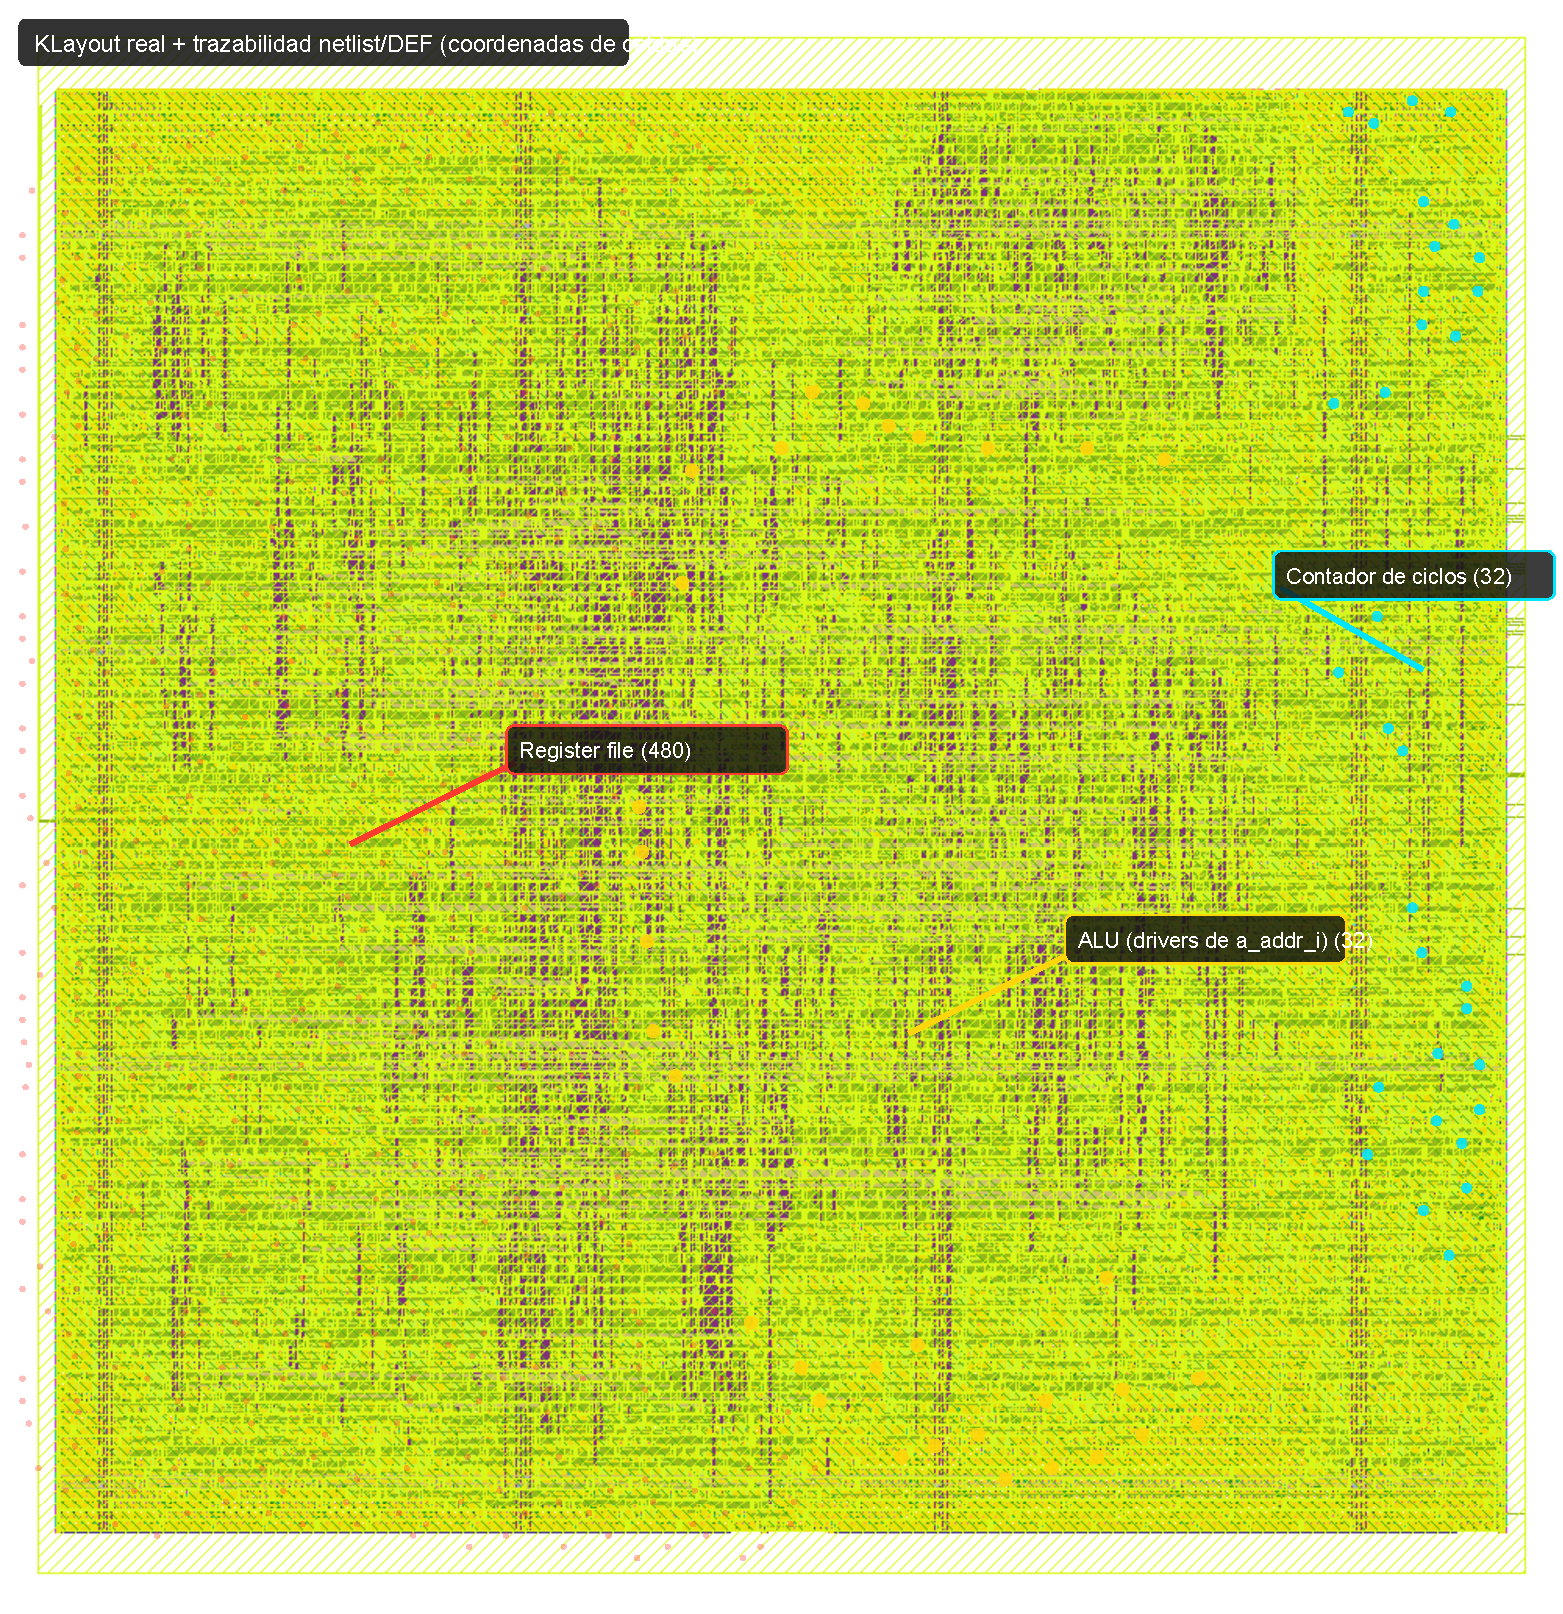
\includegraphics[width=0.94\linewidth]{figuras/etapa6_layout_trazabilidad.pdf}
\caption{Trazabilidad sobre una captura real de \ruta{etapa6_rom_ram_grt60}: el recuadro ``Register file (480)'' agrupa celdas asociadas al banco de registros; ``ALU (drivers de \ruta{a_addr_i}) (32)'' marca la frontera física observable de la ALU después del aplanamiento; y ``Contador de ciclos (32)'' identifica sus FF. Las coordenadas se obtuvieron de netlist/DEF. Es una corrida experimental, con 542/3/55 violaciones de slew/capacitancia/fanout, y no un layout eléctricamente cerrado.}
\label{fig:trace-layout}
\end{figure}

\section{Simulación RTL frente a post-síntesis}
Se simuló el netlist post-síntesis sin retardos anotados de \ruta{etapa7_rom_ram_post_synth} con modelos Verilog reales de \ruta{gf180mcu_fd_sc_mcu7t5v0}. El testbench aplica estímulos idénticos al RTL, genera VCD/logs y compara señales ciclo a ciclo. No se utilizó GDSII ni la ALU experimental.

\begin{table}[H]
\centering\small
\caption{Equivalencia RTL y post-síntesis.}
\label{tab:postsynth}
\begin{tabularx}{\linewidth}{p{0.18\linewidth}YYp{0.18\linewidth}}
\toprule
Caso & Resultado RTL & Resultado post-síntesis & Coincidencia \\
\midrule
A: ronda correcta & Objetivo 8, puntaje 1, display 00, 47 ciclos & Igual, 47 ciclos & Exacta \\
B: botón incorrecto & Objetivo 4, botón 1, EE, score 0, reinicio; 37 ciclos & Igual, 37 ciclos & Exacta \\
C: diez rondas & Score 10, promedio 01; 47,54,61,68,75,82,89,96,103,110 ciclos & Igual & Exacta; \ruta{mismatches=0} \\
\bottomrule
\end{tabularx}
\end{table}

Esto demuestra equivalencia para los estímulos cubiertos y preserva los ciclos medidos, no solamente LED. No sustituye equivalencia formal exhaustiva ni simulación post-PnR con SDF.

La tabla anterior documenta la equivalencia histórica de Etapa 7 y no se
presenta como una nueva simulación del ECO de Etapa 21. Para la corrida de
cierre \ruta{etapa21_combined} se regeneró un adaptador desde
\ruta{final/nl/asic_top.nl.v} que utiliza únicamente los puertos externos.
La comparación observable externa de 208 ciclos terminó con
\ruta{mismatches=0}; el benchmark pareado de 1008 ciclos también terminó con
\ruta{mismatches=0} en LEDs, displays y SPI. Estos resultados no cubren las
esperas reales de 30.000.000 ciclos ni las diez rondas.

\begin{table}[H]
\centering\small
\caption{Validación funcional disponible para el netlist final.}
\label{tab:stage21-functional}
\begin{tabularx}{\linewidth}{lrrY}
\toprule
Prueba & Ciclos & Diferencias & Estado \\
\midrule
Comparación externa Etapa 21 & 208 & 0 & Reset, reposo, pulso externo y salidas observables \\
Benchmark pareado & 1008 & 0 & RTL y gate-level con estímulos idénticos \\
Ronda correcta completa & -- & -- & No ejecutada: costo gate-level impracticable \\
Botón incorrecto completo & -- & -- & No ejecutada: costo gate-level impracticable \\
Diez rondas y promedio & -- & -- & No ejecutada: costo gate-level impracticable \\
\bottomrule
\end{tabularx}
\end{table}

Icarus gate-level ejecuta aproximadamente 234 ciclos/s; por ello, una ronda
completa requiere del orden de días y diez rondas del orden de semanas. Una
instalación aislada de Verilator 5.020 aceleró el RTL a aproximadamente 3,3
millones de ciclos/s, pero rechazó los UDP y las especificaciones de fuerza
de los modelos GF180MCU. No se declara equivalencia exhaustiva ni formal.

\section{Conclusiones y limitaciones}
El proyecto adaptó el RTL de FPGA a ASIC sin perder el juego de diez rondas,
implementó dos arquitecturas de memoria, incorporó el programa en hardware
sin \ruta{readmemh} y demostró equivalencia RTL/post-síntesis en los casos
probados con \ruta{mismatches=0}, incluidos los ciclos de respuesta.
La ROM combinacional con RAM reducida resultó la decisión arquitectónica
más eficiente en área y cantidad de FF frente a la memoria unificada.
El menor período demostrado para ROM+RAM fue 62\ns{} bajo las
restricciones evaluadas.

La corrida reglamentaria de 100\ns{} y 40\% (Etapa 9) conserva 2695/10/58
violaciones y se mantiene como referencia académica. Las reparaciones ECO
posteriores culminaron en \ruta{etapa21_combined}, con slew/capacitancia/
fanout = 0, setup y hold positivos en nueve corners, y DRC, LVS, antena,
XOR y KLayout externo limpios. Esta corrida es el cierre eléctrico del
macro bajo las restricciones disponibles y sustituye a Etapa 12 como mejor
candidata física, sin alterar la referencia reglamentaria.

Los GDSII de las corridas anteriores son \emph{candidatos}; la corrida
\ruta{etapa21_combined} es el candidato de macro con cierre eléctrico y físico
bajo las restricciones disponibles. No constituye una certificación de
fabricación de un chip completo con pads e I/O. La validación funcional del
juego completo en el netlist final sigue limitada por el costo de simulación;
la equivalencia demostrada corresponde a los estímulos cubiertos, no a una
equivalencia exhaustiva o formal. También faltan restricciones SDC de interfaz
ASIC basadas en cargas y delays reales: no se definieron
\ruta{PNR_SDC_FILE} ni \ruta{SIGNOFF_SDC_FILE} específicos. Deben
confirmarse la aceptación académica del deck KLayout externo y la
trazabilidad de layout de cualquier futura corrida cerrada. La
documentación pública de GF180MCU se describe como \emph{Experimental
Preview}; las verificaciones del curso no equivalen a aprobación
comercial~\cite{gf180mcu_pdk_docs}.

\appendix
\section{Reproducibilidad y evidencias}
Los comandos y rutas se documentan en \ruta{README.md} y en
\ruta{docs/proyecto3_etapa3.md} a \ruta{docs/proyecto3_etapa24.md}.
Evidencias principales:
\begin{itemize}[nosep]
\item \ruta{asic/runs/etapa9_rom_ram_util40_debounce/}: baseline reglamentaria.
\item \ruta{asic/runs/etapa4_rom_ram_100ns_*/55-openroad-stapostpnr/}: barrido de timing.
\item \ruta{reports/stage8/}: síntesis jerárquica y desglose de área.
\item \ruta{tests/stage7/}: testbench, logs y VCD post-síntesis.
\item \ruta{reports/stage9/klayout_drc_etapa9_util40/}: KLayout DRC externo.
\item \ruta{reports/stage12/} a \ruta{reports/stage21/}: comparación eléctrica, timing por corner y logs de las reparaciones dirigidas.
\item \ruta{reports/stage21/}, \ruta{reports/stage22/} y \ruta{reports/stage24/}: comparación externa, benchmarks y diagnóstico de Verilator.
\item \ruta{asic/runs/etapa21_combined/final/gds/asic_top.gds}: GDSII candidato de la corrida con cierre eléctrico del macro.
\item \ruta{asic/runs/etapa21_combined/final/nl/asic_top.nl.v} y \ruta{asic/runs/etapa21_combined/final/spef/}: netlist y SPEF de la misma implementación física.
\item \ruta{docs/proyecto3_referencias_oficiales.md}: auditoría frente a fuentes oficiales.
\end{itemize}

\bibliographystyle{plain}
\bibliography{referencias}
\end{document}
